\documentclass{chi-ext}
% Please be sure that you have the dependencies (i.e., additional LaTeX packages) to compile this example.
% See http://personales.upv.es/luileito/chiext/

%% EXAMPLE BEGIN -- HOW TO OVERRIDE THE DEFAULT COPYRIGHT STRIP -- (July 22, 2013 - Paul Baumann)
\copyrightinfo{Permission to make digital or hard copies of all or part of this work for personal or classroom use is granted without fee provided that copies are not made or distributed for profit or commercial advantage and that copies bear this notice and the full citation on the first page. Copyrights for components of this work owned by others than the author must be honoured. Abstracting with credit is permitted. To copy otherwise, or republish, to post on servers or to redistribute to lists, requires prior specific permission and/or a fee. Request permissions from the author. \\
{\emph{UWE Digital Media 2015}}, INSERT DATE, Bristol, UK.
}
% Copyright \copyright~2014 ACM ISBN/14/04...\$15.00. \\
%% EXAMPLE END -- HOW TO OVERRIDE THE DEFAULT COPYRIGHT STRIP -- (July 22, 2013 - Paul Baumann)

\title{Digital Media Ext Abstract Template: \\Note Initial Capitalisation}

\numberofauthors{6}
% Notice how author names are alternately typesetted to appear ordered in 2-column format;
% i.e., the first 4 autors on the first column and the other 4 auhors on the second column.
% Actually, it's up to you to strictly adhere to this author notation.
\author{
  \alignauthor{
  	\textbf{First Author}\\
  	\affaddr{Department of Computer Science and Creative Technology}\\
  	\affaddr{University of the West of England}\\
  	\affaddr{Coldharbour Lane, Bristol}\\
  	\email{author1@uwe.ac.uk}
  }\alignauthor{
  	\textbf{or}\\
  	\affaddr{Include student number only for}\\
  	\affaddr{anonymous submission}\\
  	\email{ }
  } 
}

% Paper metadata (use plain text, for PDF inclusion and later re-using, if desired)
\def\plaintitle{DM LaTeX Extended Abstracts Template}
\def\plainauthor{ }
\def\plainkeywords{}
\def\plaingeneralterms{}

\hypersetup{
  % Your metadata go here
  pdftitle={\plaintitle},
  pdfauthor={\plainauthor},  
  pdfkeywords={\plainkeywords},
  pdfsubject={\plaingeneralterms},
  % Quick access to color overriding:
  %citecolor=black,
  %linkcolor=black,
  %menucolor=black,
  %urlcolor=black,
}

\usepackage{graphicx}   % for EPS use the graphics package instead
\usepackage{balance}    % useful for balancing the last columns
\usepackage{bibspacing} % save vertical space in references


\begin{document}

\maketitle

\begin{abstract}
Updated 25/3/2015 and 18/09/2014.  In this sample document, we describe the formatting requirements for Digital Media Extended Abstracts, and this sample file offers recommendations on writing for the worldwide research readership. This template is based on the standard SIGCHI (Special Interest Group on Computer Human Interaction) ACM extended abstracts template.
\end{abstract}

\keywords{\plainkeywords}
Authors’ choice; of terms; separated; by semi-colons
\textcolor{red}{Optional section to be included in your final version, but strongly encouraged.}


% =============================================================================
\section{Introduction}
% =============================================================================
This format is to be used for submissions that are marking in the Digital Media  programme. We wish to give the programme a consistent, high-quality appearance and encourage students to experience writing for a wider research audience. We therefore ask that authors follow some simple guidelines. In essence, you should format your paper exactly like this document. 
The easiest way to do this is simply to download a template from the programme blackboard website and replace the example content as necessary. This template is available in Microsoft word format and latex with a .pdf version as an example. 
All submissions of complete work using this template should be in.pdf format to preserve formatting and enable marking and feedback.
The easiest way to do this is simply to download a template from the programme blackboard website and replace the example content as necessary. This template is available in Microsoft word format and latex with a .pdf version as an example. 
All submissions of complete work using this template should be in.pdf format to preserve formatting and enable marking and feedback.


% =============================================================================
\section{Text formatting}
% =============================================================================
Please use an 8.5-point Verdana font, or other sans serifs font as close as possible in appearance to Verdana in which these guidelines have been set. 
Arial 9-point font is a reasonable substitute for Verdana as it has a similar x-height. 
Please use serif or non-proportional fonts only for special purposes, such as distinguishing source code text.
Additionally, here is an example of footnoted text.\footnote{Use footnotes sparingly, if at all.}
As stated in the footnote, footnotes should rarely be used.

\subsection{Language, style, and content}
% -----------------------------------------------------------------------------
The written and spoken language of SIGCHI is English. 
Spelling and punctuation may use any dialect of English (e.g., British, Canadian, US, etc.) provided this is done consistently. 
Hyphenation is optional. 
To ensure suitability for an international audience, please pay attention to the following:

\begin{itemize}\compresslist
\item 	
Write in a straightforward style. 
Use simple sentence structure. 
Try to avoid long sentences and complex sentence structures. 
Use semicolons carefully.
\item 	
Use common and basic vocabulary (e.g., use the word ``unusual" rather than the word ``arcane").
\item 	
Briefly define or explain all technical terms. 
The terminology common to your practice/discipline may be different in other design practices/disciplines.
\item 	
Spell out all acronyms the first time they are used in your text. 
For example, ``World Wide Web (WWW)".
\item 	
Explain local references (e.g., not everyone knows all city names in a particular country).
\item 	
Explain ``insider" comments. 
Ensure that your whole audience understands any reference whose meaning you do not describe (e.g., do not assume that everyone has used a Macintosh or a particular application).
\item 	
Explain colloquial language and puns. 
Understanding phrases like ``red herring" requires a cultural knowledge of English. 
Humor and irony are difficult to translate.
\item 	
Use unambiguous forms for culturally localized concepts, such as times, dates, currencies and numbers (e.g., ``1-5-97" or ``5/1/97" may mean 5 January or 1 May, and ``seven o'clock" may mean 7:00 am or 19:00).
\item 	
Be careful with the use of gender-specific pronouns (he, she) and other gender-specific words (chairman, manpower, man-months). 
Use inclusive language (e.g., she or he, they, chair, staff, staff-hours, person-years) that is gender-neutral. 
If necessary, you may be able to use ``he" and ``she" in alternating sentences, so that the two genders occur equally often~\cite{Schwartz95}. 
\end{itemize}


% =============================================================================
\section{Figures}
% =============================================================================
The examples on this and following pages should help you get a feel for how screen-shots and other figures should be placed in the template. 
Be sure to make images large enough so the important details are legible and clear.

\begin{figure}
  \centering
  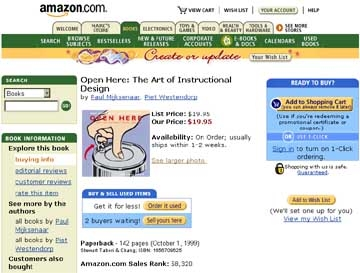
\includegraphics[width=\linewidth]{sample.jpg}
  \caption{Insert a caption below each figure.}
  \label{fig:sample}
\end{figure}
\marginpar{
\begin{figure}
  \begin{center}
  
\includegraphics[width=\marginparwidth]{Figure2.png}
  \caption{One good use of the narrow margin column: callouts that annotate a figure, either with text or a more detailed image.}
  \label{fig:marginparsample}
  \end{center}  
\end{figure}
}


Your document may use color figures, which are included in the page limit; the figures must be usable when printed in black and white.
You can use the \LaTeX's \texttt{marginpar} command to insert figures in the (left) margin side of the document (see \autoref{fig:marginparsample}).


% =============================================================================
\section{References and Citations}
% =============================================================================
Use a numbered list of references at the end of the article, ordered alphabetically by first author, and referenced by numbers in brackets \cite{Anderson92,Klemmer02,Mather00,Zellweger01}
For papers from conference proceedings, include the title of the paper and an abbreviated name of the conference (e.g., for Interact 2003 proceedings, use Proc. Interact 2003). 
Do not include the location of the conference or the exact date; do include the page numbers if available. 
See the examples of citations at the end of this document. 

Your references should be published materials accessible to the public.  
Internal technical reports may be cited only if they are easily accessible (i.e., you provide the address for obtaining the report within your citation) and may be obtained by any reader for a nominal fee.  
Proprietary information may not be cited. 
Private communications should be acknowledged in the main text, not referenced  (e.g., [Robertson, personal communication]).

% =============================================================================
\section{Producing and testing PDF files}
% =============================================================================
We recommend that you produce a PDF version of your submission well before the final deadline. 
Besides making sure that you are able to produce a PDF, you will need to check that (a) the length of the file remains within the submission category's page limit, (b) the PDF file size is 4 megabytes or less, and (c) the file can be read and printed using Adobe Acrobat Reader. 
Test your PDF file by viewing or printing it with the same software we will use when we receive it, Adobe Acrobat Reader Version 7. 
This is widely available at no cost from~\cite{Acrobat7}.  
Note that most reviewers will use a North American/European version of Acrobat reader, which cannot handle documents containing non-North American or non-European fonts (e.g. Asian fonts).  
Please therefore do not use Asian fonts, and verify this by testing with a North American/European Acrobat reader (obtainable as above). Something as minor as including a space or punctuation character in a two-byte font can render a file unreadable.

% =============================================================================
\section{Placeholder Section}
% =============================================================================
Lorem ipsum dolor sit amet, consectetur adipiscing elit. Donec a diam lectus. Sed sit amet ipsum mauris. Maecenas congue ligula ac quam viverra nec consectetur ante hendrerit. Donec et mollis dolor. Praesent et diam eget libero egestas mattis sit amet vitae augue. Nam tincidunt congue enim, ut porta lorem lacinia consectetur. \textit{Donec ut libero} sed arcu vehicula ultricies a non tortor. Lorem ipsum dolor sit amet, consectetur adipiscing elit. Aenean ut gravida lorem. Ut turpis felis, pulvinar a semper sed, adipiscing id dolor. Pellentesque auctor nisi id magna consequat sagittis. Curabitur dapibus enim sit amet elit pharetra tincidunt feugiat nisl imperdiet. Ut convallis libero in urna ultrices accumsan.

Vivamus fermentum semper porta. Nunc diam velit, adipiscing ut tristique vitae, sagittis vel odio. Maecenas convallis ullamcorper ultricies. Curabitur ornare, ligula semper consectetur sagittis, nisi diam iaculis velit, id fringilla sem nunc vel mi. Nam dictum, odio nec pretium volutpat, arcu ante placerat erat, non tristique elit urna et turpis. Quisque mi metus, ornare sit amet fermentum et, tincidunt et orci. Fusce eget orci a orci congue vestibulum. Ut dolor diam, elementum et vestibulum eu, porttitor vel elit. Curabitur venenatis pulvinar tellus gravida ornare. Sed et erat faucibus nunc euismod ultricies ut id justo. 

\subsection{Placeholder subsection}

Nullam cursus suscipit nisi, et ultrices justo sodales nec. Fusce venenatis facilisis lectus ac semper. Aliquam at massa ipsum. Quisque bibendum purus convallis nulla ultrices ultricies. Nullam aliquam, mi eu aliquam tincidunt, purus velit laoreet tortor, viverra pretium nisi quam vitae mi. Fusce vel volutpat elit. Nam sagittis nisi dui.Ut turpis felis, pulvinar a semper sed, adipiscing id dolor. 

\textbf{Mauris vitae nisi at sem facilisis semper ac in est.}

Pellentesque auctor nisi id magna consequat sagittis. Curabitur dapibus enim sit amet elit pharetra tincidunt feugiat nisl imperdiet. Ut convallis libero in urna ultrices accumsan. Donec sed odio eros. Donec viverra mi quis quam pulvinar at malesuada arcu rhoncus. Cum sociis natoque penatibus et magnis dis parturient montes, nascetur ridiculus mus. In rutrum accumsan ultricies. 


\section{Acknowledgements}
We thank all DUX 2003 publications support and staff who wrote this document originally and allowed us to modify it for this conference.
This template was based on Manas Tungare's \texttt{chi.cls}, and rewritten by Luis A. Leiva.

\section{References format}
References must be the same font size as other body text.
% REFERENCES FORMAT
% References must be the same font size as other body text.

\balance
\bibliographystyle{acm-sigchi}
\bibliography{sample}

\end{document}